\documentclass[12pt]{article}
\usepackage[british,UKenglish,USenglish,american]{babel}
\usepackage{lmodern} 
\usepackage{graphicx}
\usepackage{float}
\usepackage{pdfpages} 
\usepackage{listings}
\usepackage[colorlinks=true, urlcolor=blue, linkcolor=blue]{hyperref}
\usepackage{fancyhdr}
\usepackage{titlesec}
\usepackage{geometry}

\makeindex

\titlespacing{\chapter}{0pt}{*2}{*1.5}
\titlespacing{\section}{0pt}{*2}{*1.5}
\titlespacing{\subsection}{0pt}{*2}{*1}
\titlespacing{\subsubsection}{0pt}{*1}{*1}
\renewcommand*\familydefault{\sfdefault}
\usepackage[]{setspace}
\setstretch{1,2}

\geometry{a4paper, top=25mm, left=25mm, right=25mm, bottom=20mm,
	headsep=10mm, footskip=12mm}

\pagestyle{fancy}
\fancyhf{}
\fancyhead[R]{
\includegraphics[width=0.2\textwidth]{THM-Logo}}
\fancyhead[OL]{\thepage}
\renewcommand{\headrulewidth}{0.5pt}



\begin{document}

	\begin{titlepage}
		\centering
		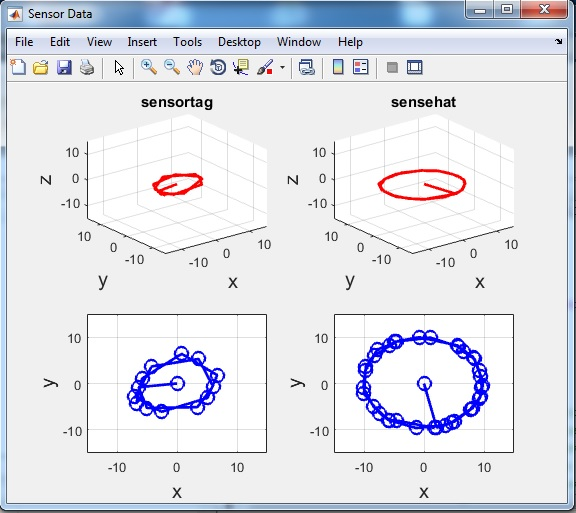
\includegraphics[width=0.5\textwidth]{Plot.jpg}\par\vspace{1cm}
		{\scshape\huge  SenseHat and SensorTag Data Processing \par}
		\vspace{1cm}
		{\scshape\Large IoT-Seminar SS2017\par}
		{\scshape\Large Authors: \par}
		\vspace{1cm}
		{\normalsize Frank L\"uhring \\ email: \href{mailto:frank.luehring@ei.thm.de}{frank.luehring@ei.thm.de}}\\
		{\normalsize Mahmoud Mansur \\ email: \href{mailto:mahmoud.mansour@iem.thm.de}{mahmoud.mansour@iem.thm.de}}\\
		{\normalsize Bj\"orn Ziegler \\ email: \href{mailto:bjoern.ziegler@ei.thm.de}{bjoern.ziegler@ei.thm.de}}    
		\vfill
		{\large \today\par}
	\end{titlepage}

\newpage
\noindent
\lstset{basicstyle=\small,
	breaklines=true,
	language=java,
	showspaces=false,
	showtabs=false}	

\tableofcontents

\newpage
\section{Introduction}

This document is the result of groups 4 work in the Internt of Things-Seminar by Prof. Dr.-Ing Birkel in the summer-semester of 2017. We had to gather in groups of two to three and work on different topics all in regards to the Internet of Things. We choose the topic:
\begin{center}
	
	SenseHat and SensorTag Data Processing
	
\end{center}
We got as further information that processing of the data have to be done in Matlab or Octave and the protocol which has to be used is the MQTT-protocol. So final task was to gather data from different sensor sources, timestamp it, and send these data with the MQTT-protocol to an MQTT-Broker. From there we import the data into Matlab and visualize it. The sensors are attached to a turning wheel to simulate the movement(see figure \ref{fig:realwheel.jpg}).We will explain the hard- and soft-ware we used, also the problems and solutions we discovered. 
This document will be more a manual for students than a technical report.  
\begin{figure}[H]
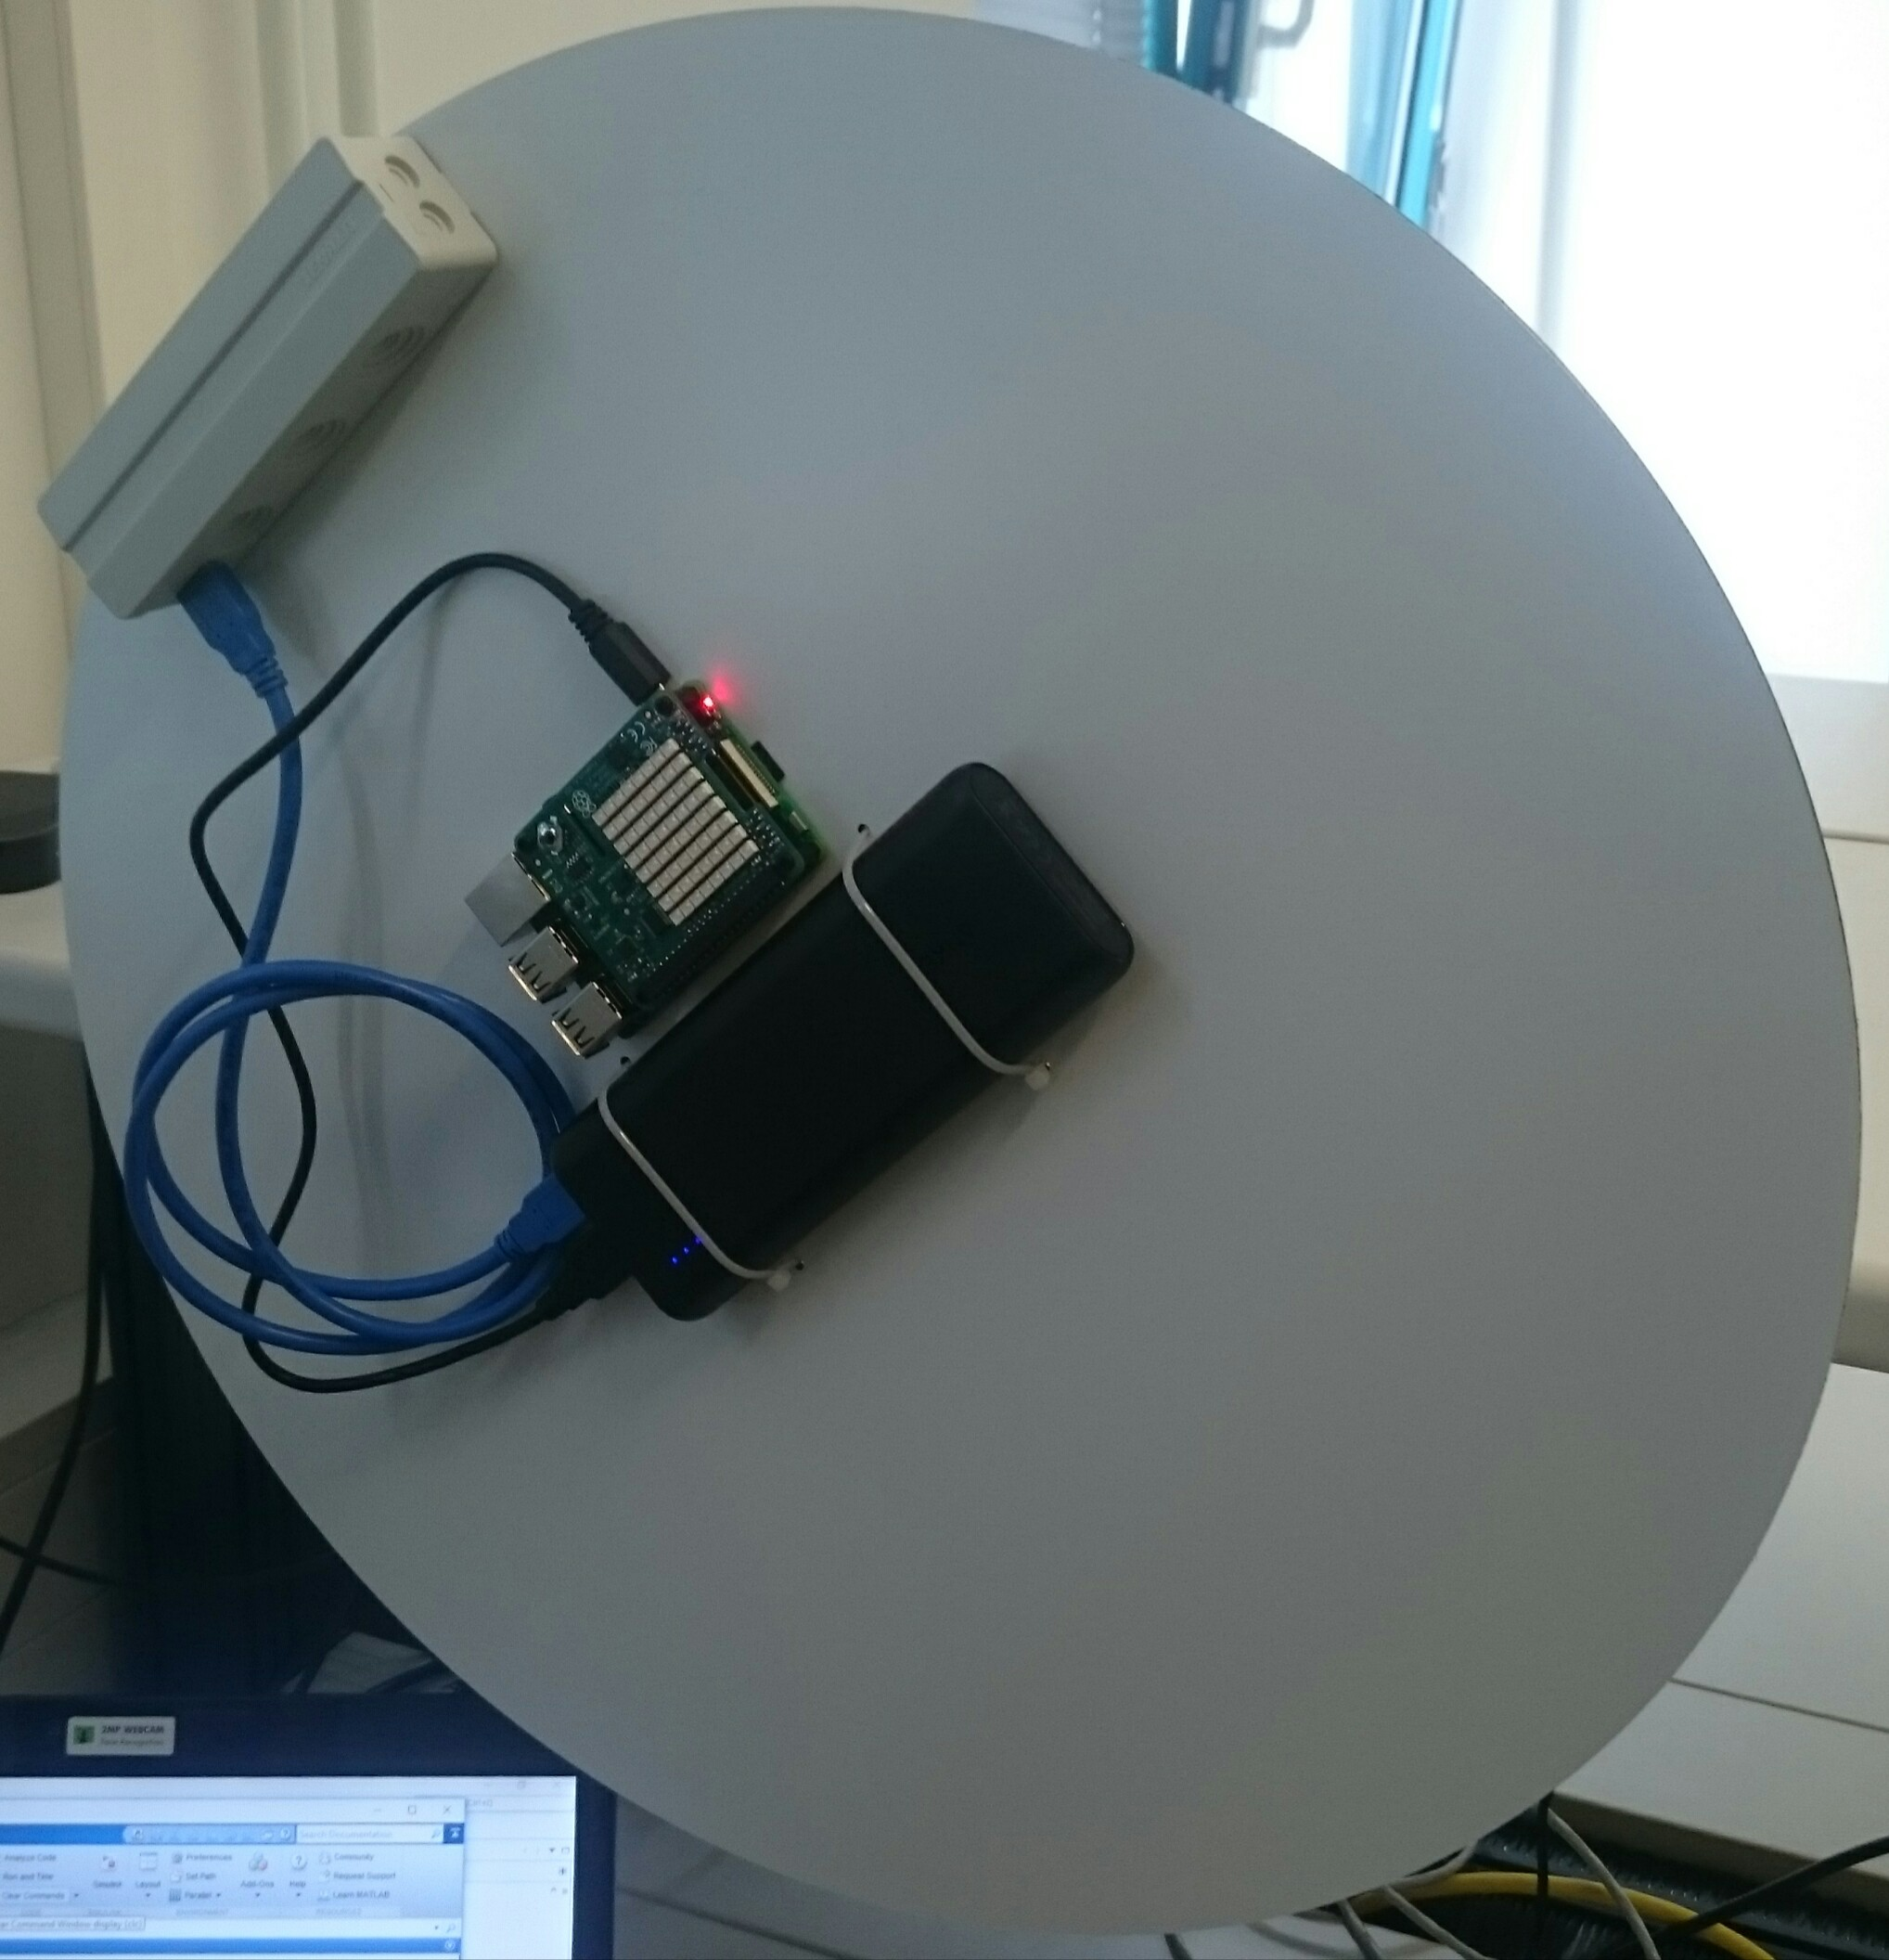
\includegraphics[width=0.5\linewidth]{realwheel.jpg}
\centering
\caption{Wheel}
\label{fig:realwheel.jpg}
\end{figure}
\newpage 
\section{Fundamentals}
In this part we are going to give you an overview over the hard- and soft-ware we used in this project. The hard- and software were placed at our disposal by the THM. Raspbian was already  installed on the raspberry pi, so we didn't have to search for a suitable OS. Every student could get a set consisting of a Raspberry Pi 3 and Sense-HAT to work at home with. Just for work at home we had to use a private license of Matlab or had to change software to octave. 
\subsection{Hardware}

\subsubsection{Raspberry Pi}
 Raspberry Pi 3 Model B released in February 2016, is bundled with on-board WiFi, Bluetooth and USB boot capabilities. As of January 2017, Raspberry Pi 3 Model B is the newest mainline Raspberry Pi. We use the Raspberry as processing unit for several sensors which we send to an MQTT-Broker. 
 
 \begin{figure}[H]
 	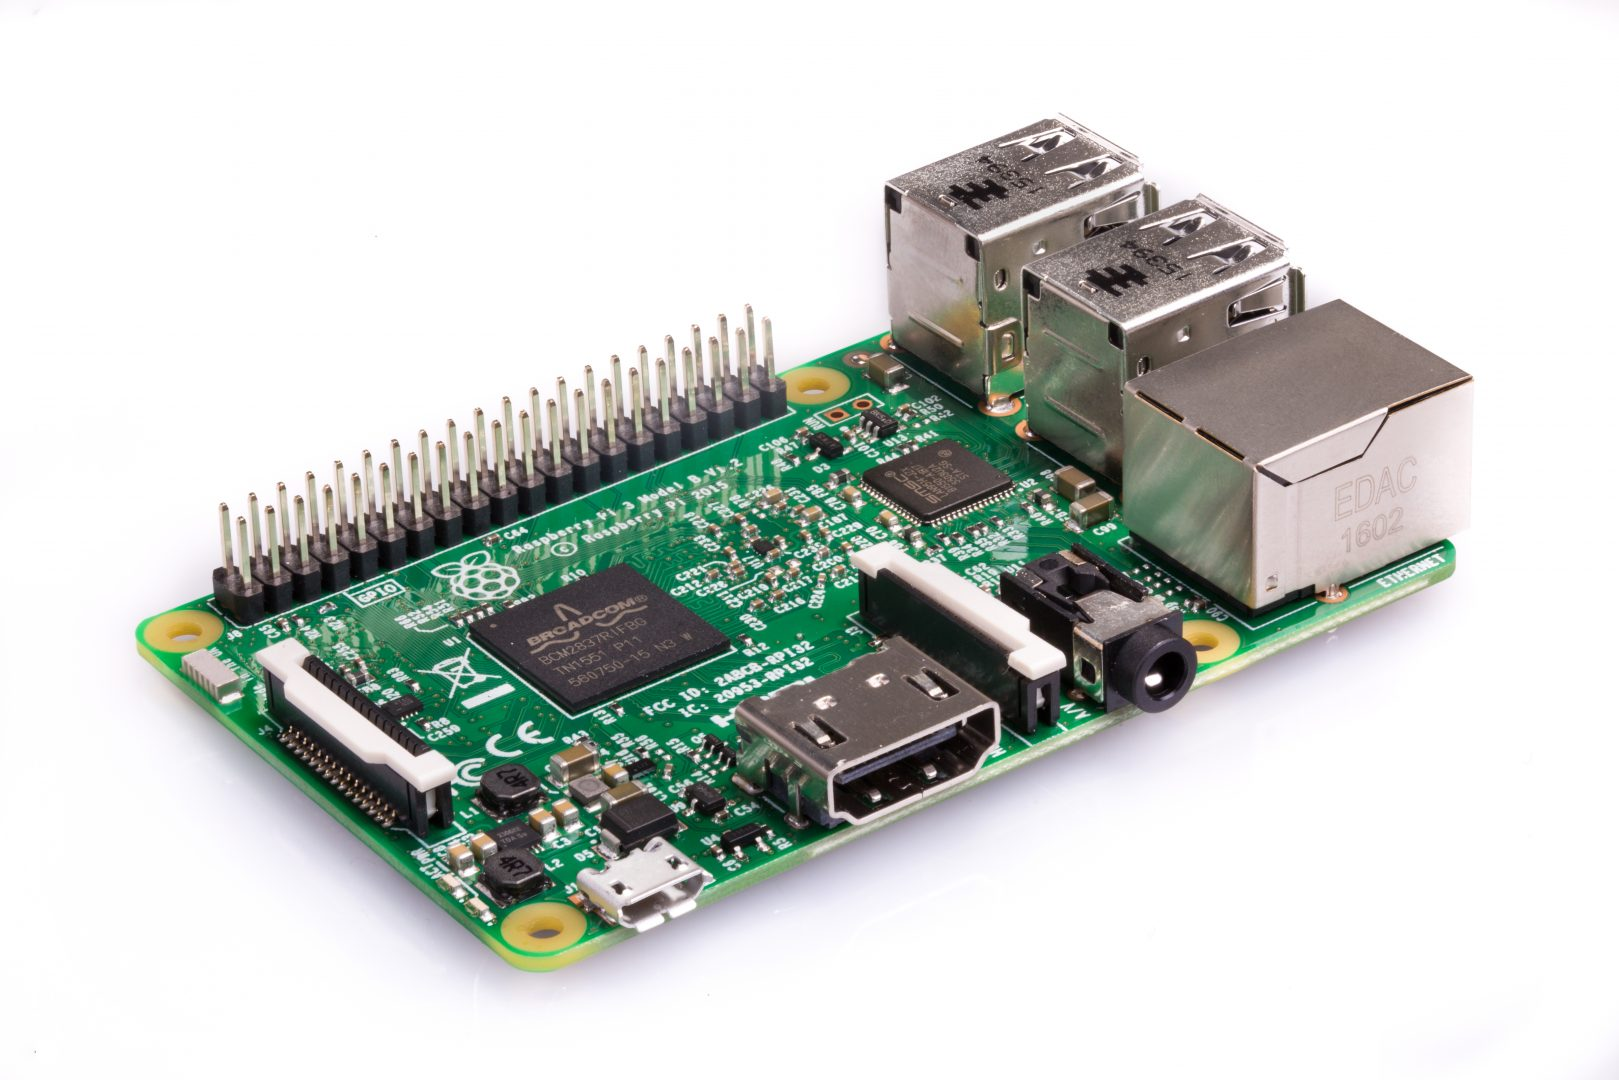
\includegraphics[width=0.7\linewidth]{Raspberry-pi-3}
 	\centering
 	\caption{Raspberry Pi 3}
 	\label{fig:raspberry-pi-3}
 \end{figure}
 
\begin{itemize}
\item SoC: Broadcom BCM2837
\item CPU: 4 x ARM Cortex-A53, 1.2GHz
\item GPU: Broadcom VideoCore IV
\item RAM: 1GB LPDDR2 (900 MHz)
\item Networking: 10/100 Ethernet, 2.4GHz 802.11n wireless
\item Bluetooth: Bluetooth 4.1 Classic, Bluetooth Low Energy
\item Storage: microSD
\item GPIO: 40-pin header, populated
\item Ports: HDMI, 3.5mm analogue audio-video jack, 4 x USB 2.0, Ethernet, Camera Serial 
\item Interface (CSI), Display Serial Interface (DSI)
\end{itemize}

\subsubsection{Sense Hat}
The Raspberry Pi Sense HAT is attached on top of the
Raspberry Pi via the 40 GPIO pins (which provids the data
and power interface) to create an "Astro Pi". For this project we use the gyroscope.

\begin{figure}[H]
	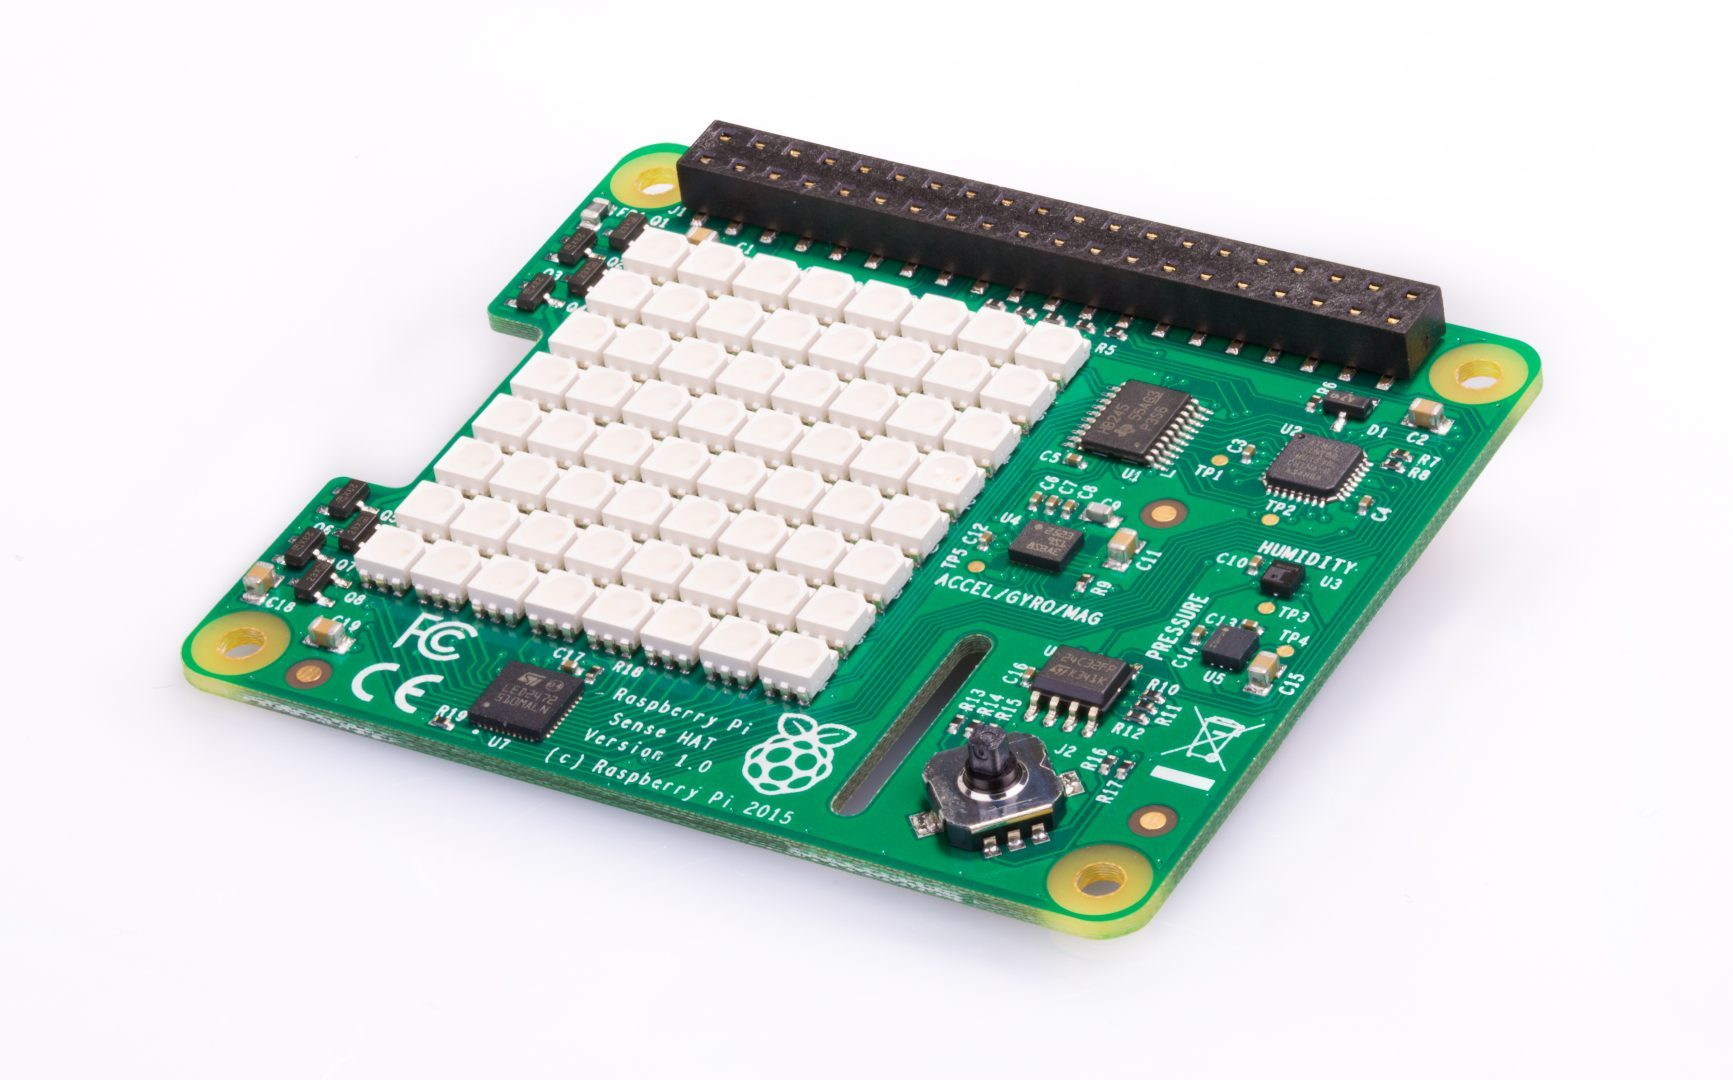
\includegraphics[width=0.7\linewidth]{Sense-HAT}
	\centering
	\caption{Sense-HAT}
	\label{fig:sense-hat}
\end{figure}

\begin{itemize}
	\item Gyroscope - angular rate sensor: $\pm$245/500/2000dps
	\item Accelerometer - Linear acceleration sensor: 2/4/8/16 g
	\item Magnetometer - Magnetic Sensor: 4/8/12/16 gauss
	\item Barometer: 260 - 1260 hPa absolute range (accuracy depends on the temperature and
	pressure, $\pm$0.1 hPa under normal conditions)
	\item Temperature sensor (Temperature accurate to $\pm$ 2$^\circ{C}$ in the 0-65$^\circ{C}$ range)
	\item 8x8 LED matrix display
	\item Small 5 button joystick
\end{itemize}

\subsubsection{Sensor Tag CC2650}

The CC2650 SimpleLink Multistandard Wireless MCU device is a wireless MCU targeting Bluetooth, ZigBee and 6LoWPAN, and ZigBee RF4CE remote control applications.
The device is a member of the CC26xx family of cost-effective, ultralow power, 2.4-GHz RF devices. Very low active RF and MCU current and low-power mode current consumption provide excellent battery
lifetime and allow for operation on small coin cell batteries and in energy-harvesting applications.

\begin{figure}[H]
	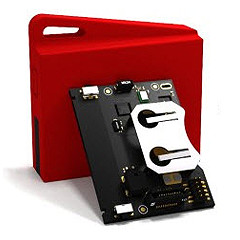
\includegraphics[width=0.5\linewidth]{CC2650.jpg}
	\centering
	\caption{Sensor Tag}
	\label{fig:cc2650}
\end{figure}


\begin{itemize}
	\item Normal Operation voltage: 1.8 to 3.8 V
	\item 10 sensors including support for light, digital microphone, magnetic sensor, humidity, pressure, accelerometer, gyroscope, magnetometer, object temperature, and ambient temperature
\end{itemize}

\subsubsection{The Wheel}
The raspberry pi with mounted Sense Hat and the Sensor Tag CC2650 are attached to a wheel like you see in figure \ref{fig:wheel}. The wheel itself is vertically attached to a small DC Motor. By powering on the power source and changing the values we can adjust the rotation speed. However, the power source and motor aren't of further interest for this project.  

\begin{figure}[H]
	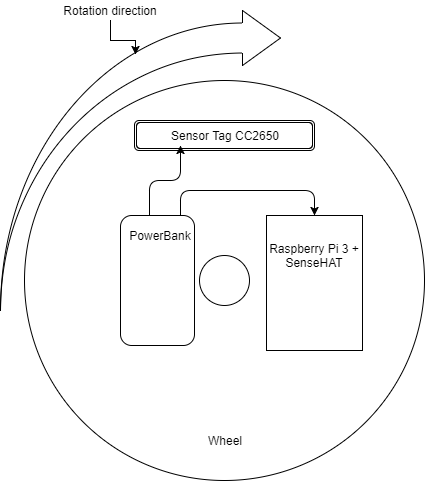
\includegraphics[width=0.7\linewidth]{wheel}
	\centering
	\caption{Wheel}
	\label{fig:wheel}
\end{figure}


\newpage

\subsection{Software}
We will give you a short overview over the Software we used in this project. This should give you shallow knowledge and a base for further investigation. 
\subsubsection{Raspbian}

Raspbian\footnote{\url{https://www.raspbian.org/}} is a free operating system based on Debian optimized for the Raspberry Pi hardware. An operating system is the set of basic programs and utilities that make your Raspberry Pi run. However, Raspbian provides more than a pure OS: it comes with over 35,000 packages, pre-compiled software bundled in a nice format for easy installation on your Raspberry Pi.
The initial build of over 35,000 Raspbian packages, optimized for best performance on the Raspberry Pi, was completed in June of 2012. However, Raspbian is still under active development with an emphasis on improving the stability and performance of as many Debian packages as possible.

\subsubsection{Node-RED}

Node-RED is a programming tool for wiring hardware devices, APIs and online services in new and interesting ways.
It provides a browser-based editor that makes it easy to wire flows using the wide range of nodes in the palette that can be deployed to its runtime in a single-click.We will explain more in chapter \ref{sec:how-to-start-node-red} and \ref{sec:Node-RED Program}.

\subsubsection{Matlab}

MATLAB\footnote{\url{https://www.mathworks.com/}} (MAtrix LABoratory) is a multi-paradigm numerical computing environment and fourth-generation programming language. A proprietary programming language developed by MathWorks, MATLAB allows matrix manipulations, plotting of functions and data, implementation of algorithms, creation of user interfaces, and interfacing with programs written in other languages, including C, C++, C\#, Java, Fortran and Python. In this project we use Java to interface with. Also we chose Matlab instead of Octave because of, in our experience, better documentation and bigger community.

\subsubsection{Java}
Java\footnote{\url{https://www.oracle.com/java/index.html}} is a general-purpose computer programming language that is concurrent, class-based, object-oriented, and specifically designed to have as few implementation dependencies as possible. It is intended to let application developers "write once, run anywhere" (WORA), meaning that compiled Java code can run on all platforms that support Java without the need for recompilation. Java applications are typically compiled to bytecode that can run on any Java virtual machine (JVM) regardless of computer architecture.
\newpage

\subsubsection{MQTT}
MQTT\footnote{\url{http://mqtt.org/}} stands for MQ Telemetry Transport, it's an simple and light messaging protocol invented in 1999 by IBM. It's designed for low-bandwidth, high latency or unreliable networks. The protocol uses a publish/subscribe architecture consisting of clients and a broker(see figure \ref{img:mqtt}). Messages in MQTT are published on topics. Topics are treated as a hierarchy, using a slash (/) as a separator. This provides a logical structure of common themes to be created. So, for example, multiple sensors can publish their position information on the following single topic, by inserting their unique sensor name: sensors/sensor\_name/position.\\
Multiple clients can then receive messages by creating a subscription to this specific topic. However, there are two wildcards available + or \#. The + character can be used as a wildcard for a single level of hierarchy.\\
The \# character can be used as a wildcard for all remaining levels of hierarchy, which means that it must be the final character in a subscription in order to match.

\begin{figure}[H]
	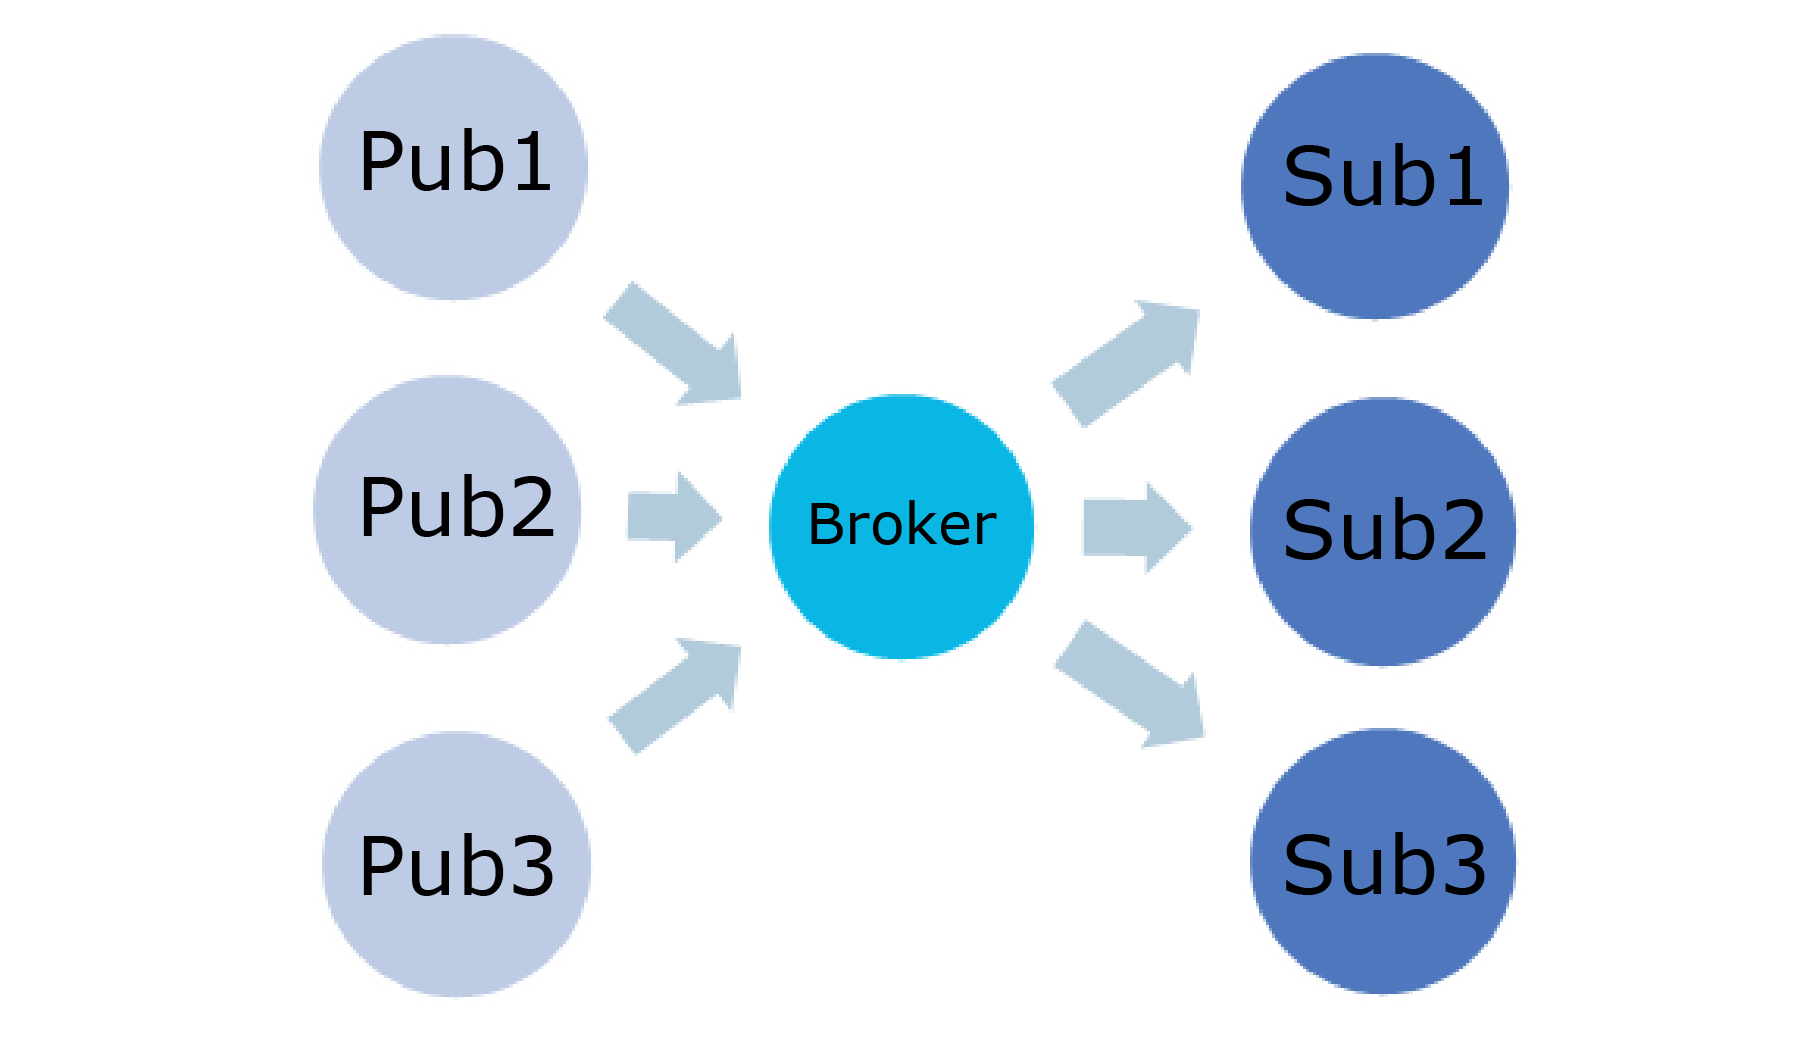
\includegraphics[width=\textwidth]{mqtt.png}
	\caption{MQTT} 
	\label{img:mqtt}	
\end{figure}

\newpage

\section{Implementation}
In this part we explain how we put the programs and hardware into operation. All code we use that aren't in this section can be found in the attachment. It will start with the programming tool node-red which runs on the raspberry. After that we will explain the Matlab code an it's functionality. More info about how to run Java-code in Matlab can be found in the attachment\ref{sec:attachment}.

\subsection{How to start node-red}\label{sec:how-to-start-node-red}
To start node-red on the raspberry pi you have to download a program like PuTTY 
\footnote{\url{http://www.putty.org/}} and connect to the raspberry pi on port 22
(See figure \ref{img:putty_conf}: PuTTY config). Login with:

\begin{itemize}
	\item user: pi
	\item password: raspberry
\end{itemize}

\begin{figure}[H]
	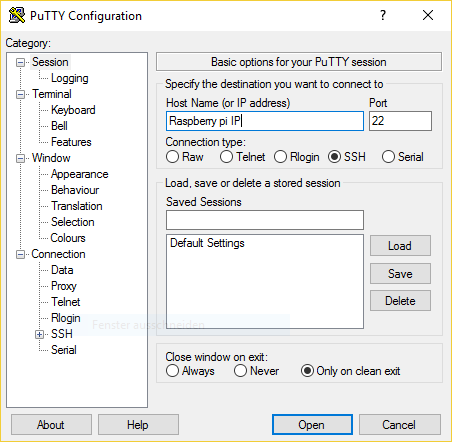
\includegraphics[width=0.5\linewidth]{putty_conf.png}
	\centering
	\caption{PuTTY config} 
	\label{img:putty_conf}	
\end{figure}
You have to change the default password if you don't work in a safe environment!\\
To Upgrade Node-Red to up-to-date version enter following commands into the command line(See figure \ref{img:putty_start_node_red}: Start nodered).

\begin{itemize}
	\item update-nodejs-and-nodered
	\item sudo systemctl enable nodered.service
	\item node-red-start
\end{itemize}

\begin{figure}[H]
    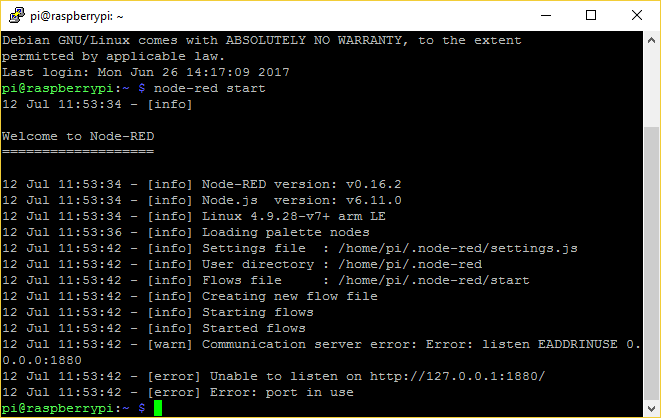
\includegraphics[width=1\textwidth]{putty_start_node_red.PNG}
    \centering
	\caption{Start nodered}
	\label{img:putty_start_node_red}
\end{figure}
Check if node-red is running by entering -ip of your raspberry pi:1880- into the adress bar of your browser. Be sure to enter the port number, otherwise it won't work. If you get displayed a website like shown in figure \ref{img:Node RED} you have successful started node-red. You are now able to compile a program! (See chapter \ref{sec:Node-RED Program})

\begin{figure}[H]
	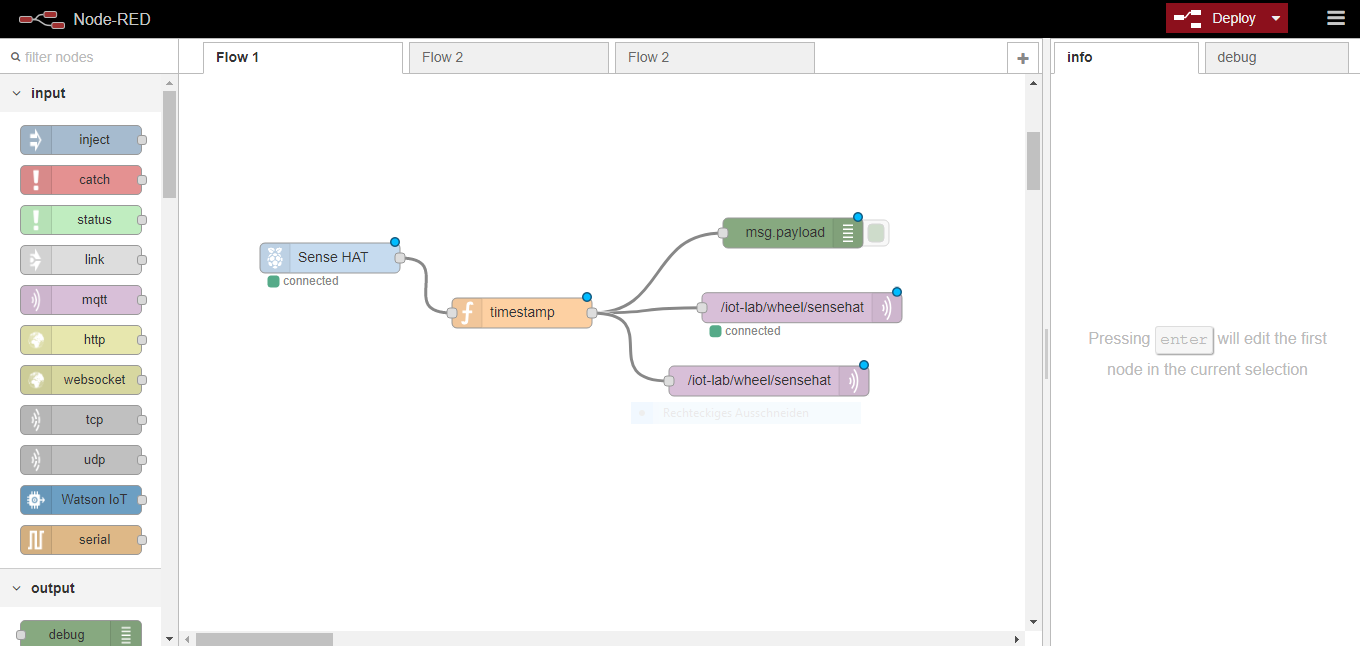
\includegraphics[width=\textwidth]{Node_red_1.PNG}
	\caption{Node RED}
	\label{img:Node RED}
\end{figure}

\newpage

\subsection{Node-RED Program}\label{sec:Node-RED Program}
Node-RED \footnote{\url{https://nodered.org/}} works with functional blocks which you can add, delete and connect by Drag'n'Drop. In figure \ref{img:Node RED} you see our program to get the data from the Sense HAT which is connected directly to the raspberry pi, timestamp it, and send it out to two MQTT-Brokers and a debug node. One click on deploy in the upper right corner compiles your program. It will appear gray after the deploy, and will turn back to red if any changes are done to the program. The Node-red code can be imported with the source code attached in \ref{sec:source-code-node-red}

\subsubsection{Sense HAT node}
The first node you see in figure \ref{img:Node RED} is the Sense HAT node. This is a premade node wich supports the Sense-HAT. Here we choose the data we need, in our case these are the motion events. Environment and joystick events aren't necessary for our purpose, so we uncheck these two points, to decrease the data traffic. 

\begin{figure}[H]
	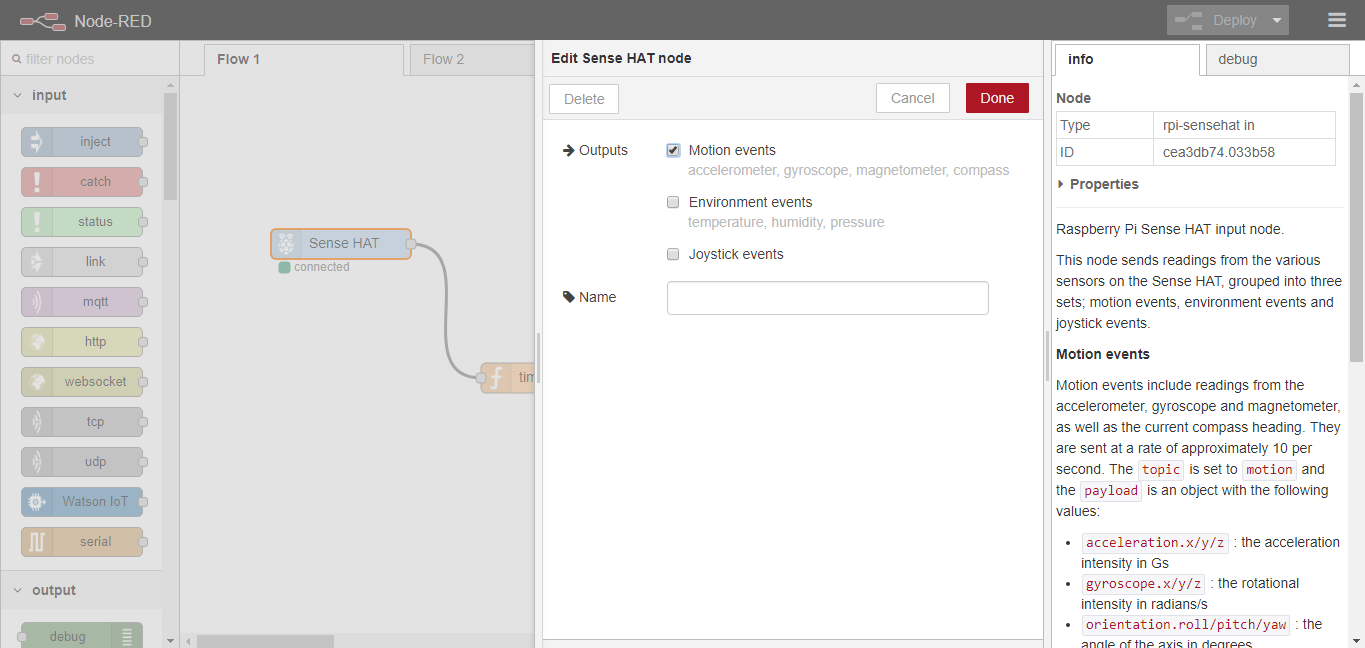
\includegraphics[width=\textwidth]{Sense_Hat_node.PNG}
	\caption{Sense HAT node}
	\label{img:Sense_Hat_node}
\end{figure}

\subsubsection{Function node}
For our purpose in Matlab we need an timestamp, to display and process the data correctly which we get from the sensors. Because we haven't found a suitable node, we had to write our own node.\ref{sec:source-code-timesptamp-node} Therefor we used the function block, named it timestamp and entered the code in JavaScript, See figure \ref{img:timestamp_function_node_red.PNG}. 

\begin{figure}[H]
	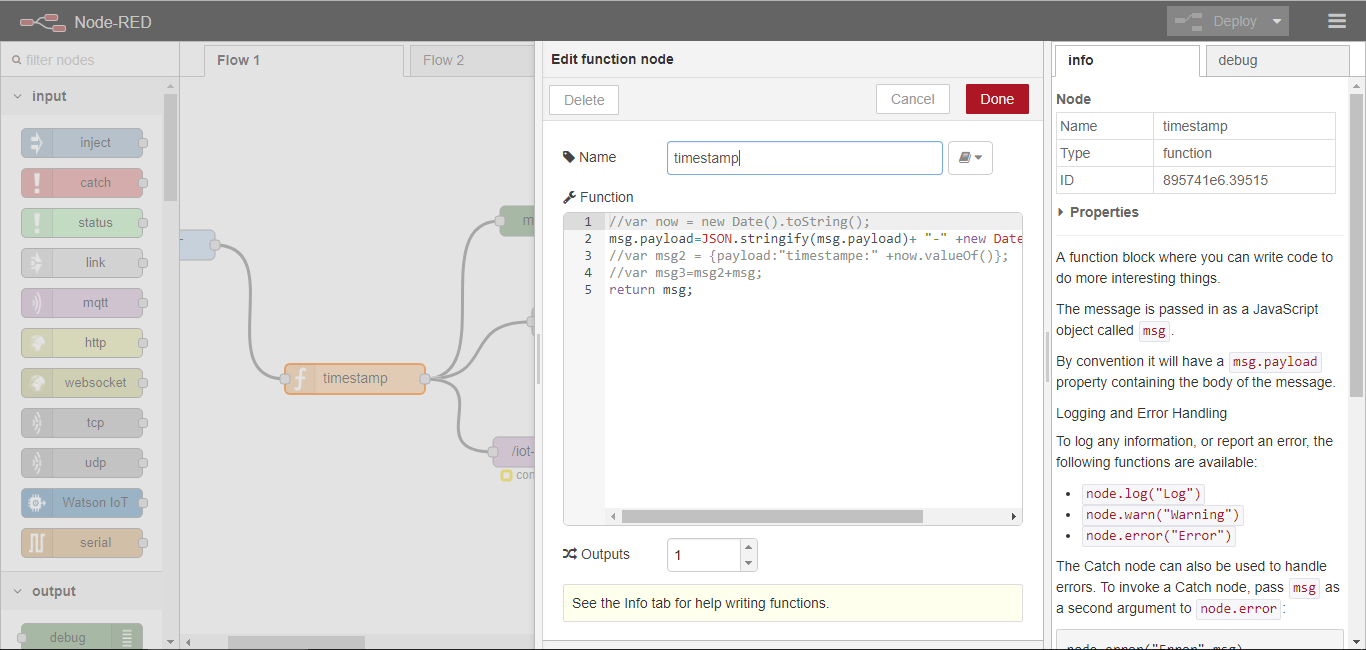
\includegraphics[width=\textwidth]{timestamp_function_node_red.PNG}
	\caption{Timestamp node}
	\label{img:timestamp_function_node_red.PNG}
\end{figure}

\subsubsection{MQTT node}
The MQTT out node is provided by Node RED. It's a node to send data with the MQTT protocol. 
	\begin{itemize}
		\item Server\newline
		Here you enter the IP or URL of your desired MQTT-Broker. For both port 1883 is used. 
		Here is a small list of online-broker we used:
		\subitem 10.24.3.66:1883 (THM local broker)
		\subitem iot.eclipse.org			
		\subitem broker.dashboard.com		
		\subitem test.mosquitto.org			
		\subitem broker.hivemq.com		
		\subitem test.mosca.io		
		\item Topic\newline
		Here you can enter a topic under which you can subscribe again to get data from. We choose for simplification /iot-lab/wheel/sensehat
		\item QoS\newline
		You have the possibility to choose between three kinds of Qualitiy of Service:
		\subitem QoS 0 - at most once
		\subitem Level zero guarantees a best effort of delivery. A message won't be 
		\subitem acknowledged or stored by an Broker. Often called "fire and forget"
		\subitem QoS 1 - at least once
		\subitem Level one guarantees that the message will be delivered at least  
		\subitem once to the Broker. The sender will wait for an acknowledgement 
		\subitem from the receiver. 
		\subitem QoS 2 - once
		\subitem The highest QoS is 2, it guarantees that each message is received 
		\subitem only once by the counterpart. It is the safest and
		\subitem  also the slowest quality of service level.
		\item Retain\newline
		A retained message is a normal MQTT message with the retained flag set to true. The broker will store the last retained message and the corresponding QoS for that topic. Each client that subscribes to a topic pattern, which matches the topic of the retained message, will receive the message immediately after subscribing.
	\end{itemize}  

\begin{figure}[H]
	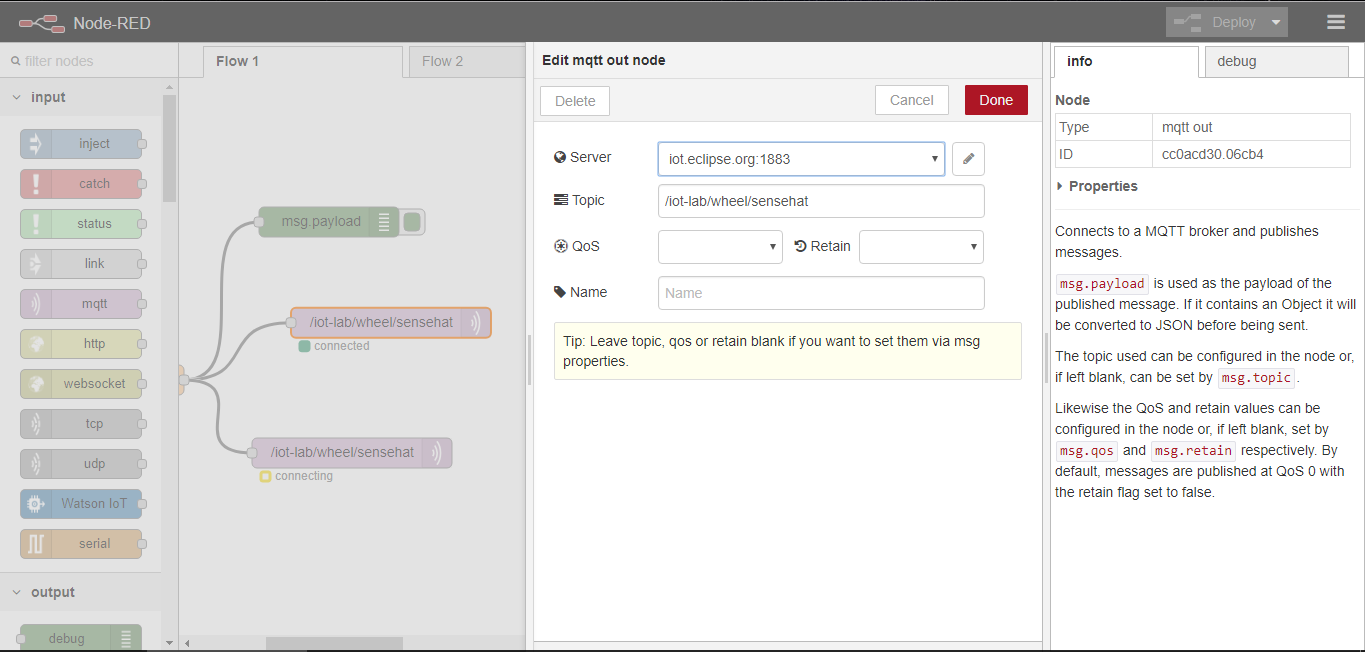
\includegraphics[width=\textwidth]{mqtt_node.PNG}
	\caption{MQTT node}
	\label{img:mqtt_node.PNG}
\end{figure}

\newpage

\subsection{Matlab}
In the previous part we explained how we get the data from the Raspberry pi to the MQTT-Broker. In this part we will illuminate how we import the data into matlab and visualize it.
\subsubsection{Important commands for Matlab}
We will explain some important commands we used and found for Matlab which are not imperative coherent to our project and are not explained anywhere else in this document, but may be of use for future projects.
\newline
javaclasspath('-dynamic')
\newline
\fbox{\begin{minipage}{35em}
		Displays the current dynamic path
\end{minipage}}
\newline
t = Matlab\_MQTT\_Client\_Main\_Class;
\newline
\fbox{\begin{minipage}{35em}
	Creates a new java instance.
\end{minipage}}
\newline
t.Subscribe(u);
\newline
\fbox{\begin{minipage}{35em}
This command is not valid in Matlab without creating a Java instance "t". This is how to call a Java method in Matlab, using a Java syntax. "t" could be a Java object or the name of the class. "Subscribe(u)" is our method in Java to subscribe to a topic.
\end{minipage}}
\newline
u = {'/iot-lab/wheel/sensehat','2'};
\newline
\fbox{\begin{minipage}{35em}
	Creates a cell array with two columns, one for the topic and one for the QoS.
\end{minipage}}
\newline
r = reshape(n,1,[]);\footnote{\url{https://de.mathworks.com/help/matlab/ref/reshape.html}}
\newline
\fbox{\begin{minipage}{35em}
		From its name, this command will reshape the dimensions of your array. If you have for instance an array with 10 rows and 1 column (10x1 = 10 elements), you could reshape it to 5 rows and 2 columns (5x2 = 10 elements). In our example the array n carries the message payload and it has always 1 column and number of its rows differ in each iterate, so we would like change it to 1 row and we write these square brackets to let Matlab choose the number of its columns
\end{minipage}}
a = native2unicode( r );\footnote{\url{https://de.mathworks.com/help/matlab/ref/native2unicode.html}} 	/ r = unicode2native ( a );\footnote{\url{https://de.mathworks.com/help/matlab/ref/unicode2native.html}}
\newline
\fbox{\begin{minipage}{35em}
		These two command convert your array from ASCII code to Unicode character and vice versa.
\end{minipage}}
\newline
w =  strsplit (a, '/') ;\footnote{\url{https://de.mathworks.com/help/matlab/ref/strsplit.html}}
\newline
\fbox{\begin{minipage}{35em}
		Matlab will split the string ( a ) into substrings when it finds the delimiter ( / ).
\end{minipage}}
\newline
[ theta2 , rho2 , z2 ] = c a r t 2 p o l ( x2 , y2 , z2 ) ;\footnote{\url{https://de.mathworks.com/help/matlab/ref/cart2pol.html}}
\newline
\fbox{\begin{minipage}{35em}
		Converting from the Cartesian coordination to polar.
\end{minipage}}
\newpage
n= t.get\_message\_(u);
\newline
\fbox{\begin{minipage}{35em}
This command are not valid in Matlab without creating your Java instance "t". This is how to call a Java method in Matlab using a Java syntax."t" could be a Java object or the name of the class. "get\_message\_(u)" is our method in Java to fetch the messages coming under a topic defined in the argument "u". If you are not subscribing to any topic, the method will return an empty array.
This method will return the last received message, in format of a byte array ( int8 column vector).
In our example, we are send a string of characters with the Sense-HAT node which we receive as a byte array. Each byte represents one character in ASCII format:
If the message at node-red was like that:\newline
"acceleration":{"x":-0.0015,"y":0.0269,"z":0.9831},"gyroscope":{"x":-0.0024,"y":-0.0016,"z":0.0002},"orientation":{"roll":1.6198,"pitch":0.0462,"yaw":245.0466}, "compass":245
\newline
You will get a an ASCII format in Matlab as a vertical array ( 216 X 1 ). Like the following:
[123, 34, 97, 99, 99, 101, 108, 101, 114, 97, 116, 105, 111, 110, 34, 58, 123, 34, etc
In the ASCII table\footnote{\url{www.theasciicode.com.ar}} each number of the previous ones meets a character. 
Numbers from 0 - 9 , the dot , and the minus symbol could be what you are looking for.
Here are the values of the characters:
\begin{itemize}
\item ascii code	45	-	(Hyphen)			
\item ascii code	46	.	(Full stop , dot)				
\item ascii code	48	0	(number zero)			
\item ascii code	49	1	(number one)			
\item ascii code	50	2	(number two)			
\item ascii code	51	3	(number three)			
\item ascii code	52	4	(number four)			
\item ascii code	53	5	(number five)			
\item ascii code	54	6	(number six)			
\item ascii code	55	7	(number seven)			
\item ascii code	56	8	(number eight)			
\item ascii code	57	9	(number nine)	
\end{itemize}
\end{minipage}}
\newpage
\subsubsection{Startup}
This is the Startup Script. It starts the GUI\footnote{graphical user interface}, like you see in figure \ref{img:GUI.PNG} to connect to the MQTT-Broker. You will find the source code for the GUI under point \ref{sec:source-code-gui}.
The command javaaddpath must point to the java file.
Insert the Server address and choose the configuration then press connect to connect to the broker.
The Matlab-code for Startup:
\lstset{basicstyle=\small,
	breaklines=true,
	language=java,
	showspaces=false,
	showtabs=false}
\newline
clear\footnote{\url{https://de.mathworks.com/help/matlab/ref/clear.html}}
\newline
\fbox{\begin{minipage}{35em}
		Clears all the variables stored in the workspace.
\end{minipage}}
\newline
clear java;
\newline
\fbox{\begin{minipage}{35em}
		Removes any dynamic entry to the dynamic path.
\end{minipage}}
\newline
javaaddpath\textit{'C:/IoT/wheel/code\_V1.4/java/dist/testmatlab5\_1\_1\_2.jar';}\footnote{\url{https://de.mathworks.com/help/matlab/ref/javaaddpath.html}}\newline
\fbox{\begin{minipage}{35em}
		Adds a java .class / .jar file to the environment.
\end{minipage}}
\newline
wheelGUI = Matlab\_MQTT\_Client\_Main\_Class;
\newline
\fbox{\begin{minipage}{35em}
		Calls the graphical user interface
\end{minipage}}
\newline
javaMethod('main',wheelGUI,'');\footnote{\url{https://de.mathworks.com/help/matlab/ref/javamethod.html}}
\newline
\fbox{\begin{minipage}{35em}
		After creating your java instance, you have to call the main Method to run your java application. Actually, this command works for any method you want to call. It is matlab syntax.
\end{minipage}}

\begin{figure}[H]
	\centering
	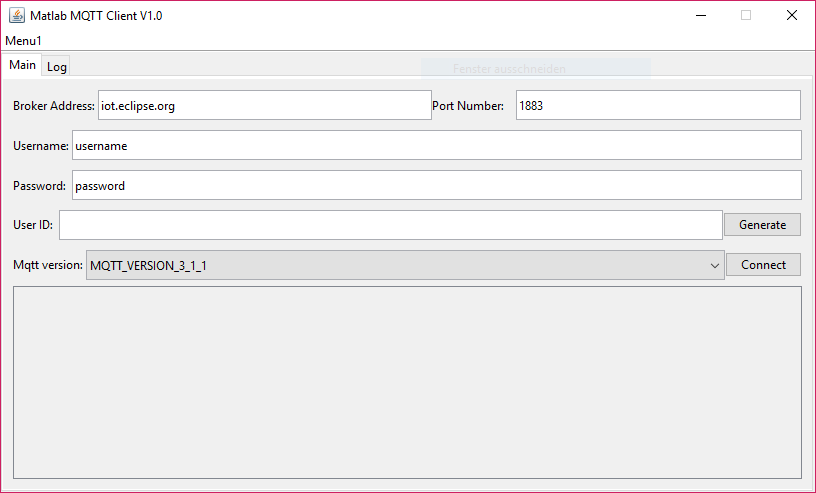
\includegraphics[width=0.7\textwidth]{GUI.PNG}
	\caption{GUI}
	\label{img:GUI.PNG}
\end{figure}
Note: Don't close the GUI, it will close Matlab aswell.

\subsubsection{Subscribe}
This is the Matlab code for subscribing to one or more brokers. 
You can change the number of strings you would connect to. You are free to add or delete connections if you need different ones.
You can see now the subscribed Topics in the GUI by selecting the Log tab. You can select the Topics and see what data you get from the sensors.(See figure \ref{img:GUI-LOG.PNG})\newline
The wheel\_subscribe.m-code:
\lstset{basicstyle=\small,
	breaklines=true,
	language=java,
	showspaces=false,
	showtabs=false}
\begin{lstlisting}
subscribes=["/iot-lab/wheel2/sensehat2","2";
		"iot_lab/wheel/sensortag","2"];
wheelGUI.Subscribe(subscribes(1,:));
wheelGUI.Subscribe(subscribes(2,:));
numberOfSubscribes=numel(subscribes)/2;
\end{lstlisting}
\begin{figure}[H]
	\centering
	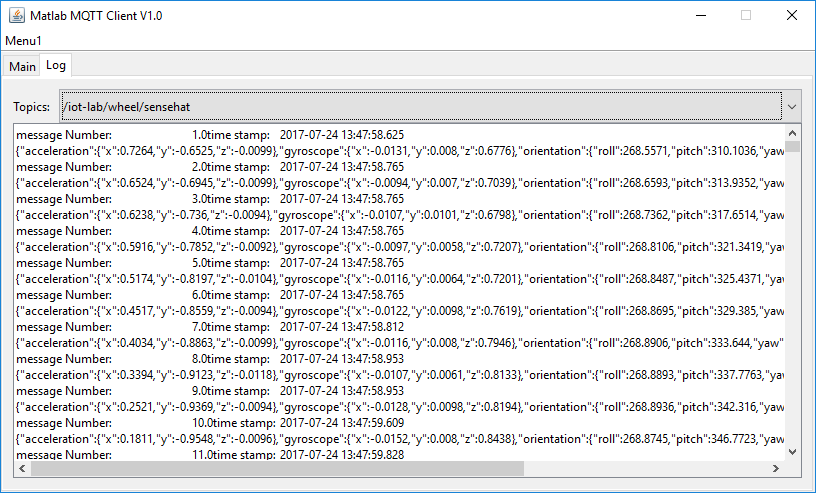
\includegraphics[width=1\textwidth]{GUI-LOG.PNG}
	\caption{GUI-Log}
	\label{img:GUI-LOG.PNG}
\end{figure}

\subsubsection{Plot}
The Plot-Code is the main-code in our data processing. Therefore we are going to explain the code more exact. In the following you will see the code itself, with explanation in the boxes.
\newline
\newline MAIN-CODE:
\lstset{basicstyle=\small,
	breaklines=true,
	language=java,
	showspaces=false,
	showtabs=false}
\begin{lstlisting}

xvec=[];
yvec=[];
zvec=[];
figure('Name','Sensor Data','NumberTitle','off');
line_wid              = 2;
FontSize              = 15;
marker_size           = 10;
buffer_length         = 100;
\end{lstlisting}
\fbox{\begin{minipage}{35em}
The following examples demonstrate all the possible Methods and Fields
in java code that you could use in matlab:
t.get\_message\_(...) \begin{itemize}
	\item receiving a MQTT message. The argument is your MQTT topic.
\end{itemize}
\end{minipage}}
\begin{lstlisting}
while true
 coordmat        = zeros(buffer_length,3);
 coordmat2       = zeros(buffer_length,3);
 for buff_index  = 1:buffer_length
	coord_vec    = [];
	coord_vec2   = [];
	pause (0.05);

	if wheelGUI.get_message_(subscribes(2,:))~=0
	 m = wheelGUI.get_message_(subscribes(2,:));

	 e = reshape(m,1,[]);
	 a = native2unicode(e);
	 c = strsplit(a,' ');
 	 x=strrep(c(2),';','');
	 x=str2double(x)/5-7.5;
	 x=x*-1;
	 y=strrep(c(4),';','');
	 y=str2double(y)/5-5;
	 z=strrep(c(6),';','');
	 z=str2double(z)/5-7.5;
	 \end{lstlisting}
	 \fbox{\begin{minipage}{35em}
	 		We multiply the value we get by the sensor so we can visualize it in a proper way. 
	 \end{minipage}}
	 \begin{lstlisting}
	else
	 x=0;
 	 y=0;
 	 z=0;
 	 \end{lstlisting}
 	 \fbox{\begin{minipage}{35em}
 	 		\centering
 	 		If no sensor data is available, the values are set to zero to prevent an error.
 	 \end{minipage}}
 	 \begin{lstlisting}
	end
	 x = round(x,1, 'decimals');
 	 y = round(y,1, 'decimals');
	 z = round(z,1, 'decimals');
\end{lstlisting}
\fbox{\begin{minipage}{35em}
	The value is rounded to two decimal figures and converted into Cartesian and polar coordinates.
\end{minipage}}
\begin{lstlisting}
	 coord_vec      = [x,y,z];  
	 [theta,rho,z]  = cart2pol(x,y,z);
\end{lstlisting}
\fbox{\begin{minipage}{35em}
	coordmat is a matrix representing the buffer where the data is stored.	
\end{minipage}}
\begin{lstlisting}
	 coordmat(buff_index,1:3) = coord_vec;
\end{lstlisting}
\fbox{\begin{minipage}{35em}
		\centering
		Sensortag-Plot	
\end{minipage}}
\begin{lstlisting}	    
	subplot(2,2,1)
	
	 plot3(coordmat(:,1),coordmat(:,2),coordmat(:,3),'r','linewidth',line_wid);
	 grid on;
	 xlim([-15 15]);ylim([-15 15]);zlim([-15 15]);
	 Xlab= xlabel('x'); Ylab=ylabel('y');Zlab=zlabel('z');
	 set(Xlab, 'FontSize', FontSize);
	 set(Ylab, 'FontSize', FontSize);
	 set(Zlab, 'FontSize', FontSize);
	 title("sensortag")
\end{lstlisting}
\fbox{\begin{minipage}{35em}
		Above we see the commands for the 3D-Plot with X,Y and Z direction
\end{minipage}}
\begin{lstlisting}	    
	subplot(2,2,3)
	
	 plot(coordmat(:,1),coordmat(:,2),'b','markersize',marker_size,'marker','o','linewidth',line_wid);
	 grid on;    
	 xlim([-15 15]);ylim([-15 15]);
	 Xlab= xlabel('x'); Ylab=ylabel('y');
	 set(Xlab, 'FontSize', FontSize);
	 set(Ylab, 'FontSize', FontSize);
	 
 \end{lstlisting}
 \fbox{\begin{minipage}{35em}
 		Above we see commands the for the 2D-Plot with X and Y direction, the following part below is nearly the same as before so we will not explain again. 
 \end{minipage}}
 \begin{lstlisting}	
	if wheelGUI.get_message_(subscribes(1,:))~=0
	 n= wheelGUI.get_message_(subscribes(1,:));
	
	 e2 = reshape(n,1,[]);
	 v2 = native2unicode(e2);
	 r2=strrep(v2,':','');
	 c2 = strsplit(r2,'"');
	 if strcmp(c2(2),'acceleration')
 	 x2=str2double(c2(5))*10;
	 y2=str2double(c2(7))*10;
	 z2=c2(9);
	 z2 = strrep(z2,'},','');
	 z2=str2double(z2)*10;
	else
	 x=0;
	 y=0;
	 z=0;
	end
	end
	 x2 = round(x2,1, 'decimals');
	 y2 = round(y2,1, 'decimals');
	 z2 = round(z2,1, 'decimals');    
	coord_vec2      = [x2,y2,z2];  
	[theta2,rho2,z2]  = cart2pol(x2,y2,z2);       
	coordmat2(buff_index,1:3) = coord_vec2;
\end{lstlisting}
\fbox{\begin{minipage}{35em}
		\centering
		Sense-HAT-Plot	
\end{minipage}}
\begin{lstlisting}

	subplot(2,2,2)

	 plot3(coordmat2(:,1),coordmat2(:,2),coordmat2(:,3),'r','linewidth',line_wid);
	 grid on;
	 xlim([-15 15]);ylim([-15 15]);zlim([-15 15]);
	 Xlab= xlabel('x'); Ylab=ylabel('y');Zlab=zlabel('z');
	 set(Xlab, 'FontSize', FontSize);
	 set(Ylab, 'FontSize', FontSize);
	 set(Zlab, 'FontSize', FontSize);    
	 title("sensehat")

	subplot(2,2,4)

	 plot(coordmat2(:,1),coordmat2(:,2),'b','markersize',marker_size,'marker','o','linewidth',line_wid);
	 grid on;    
	 xlim([-15 15]);ylim([-15 15]);
	 Xlab= xlabel('x'); Ylab=ylabel('y');
	 set(Xlab, 'FontSize', FontSize);
	 set(Ylab, 'FontSize', FontSize);
	end        
end

\end{lstlisting}

So if you successfully started and subscribed, the result should look like shown in figure \ref{fig:Plot2.jpg}.
In the top-area we have the the 3D-plots of the two sensors we are using. Right beneath we have the plots in X and Y direction, consequently the 2D-plot. This matlab script is just working for these exactly sensors. If you like to change the sensors, or the values you want to process, this part has to be changed!
\begin{figure}[H]
	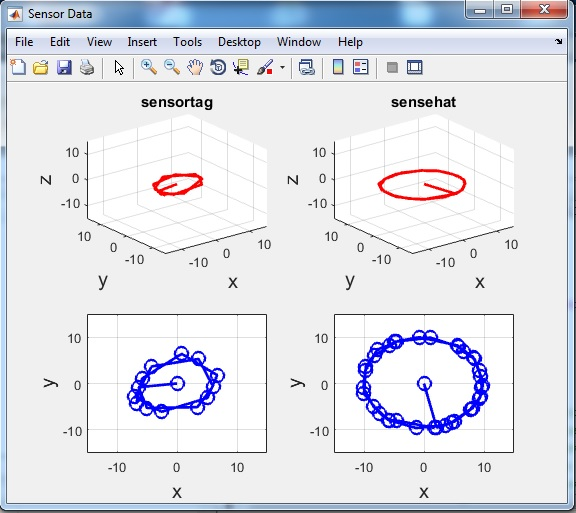
\includegraphics[width=0.5\linewidth]{Plot.jpg}
	\centering
	\caption{Plot}
	\label{fig:Plot2.jpg}
\end{figure}

\section{Summary and Conclusion}
\subsection{Summary}
This report presents a possibility to transport data with the MQTT-Protocol from different sensors, in our case the Sense-HAT and the TI SensorTag, to a MQTT-Broker and import these data into Matlab by subscribing to the Broker. First of all we look for a solution to the implementation of the MQTT-Client into Matlab. For this purpose we choose the eclipse paho open-source client implementatin. It supports MQTT and MQTT-SN messaging protocols aimed for the Internet of Things. The libraries for the implementation are available for different programming languages like C, C++, Java, JavaScript and several more. In regards to our knowledge we choose Java as a fitting language - even tough it took us some time to get Java running in Matlab. The major issues and how to treat them are explained in the attachment (see: \ref{sec:how-to-setup-java-in-matlab} and \ref{sec:how-to-add-java-class-to-matlab}). When the transmission of the data with the MQTT-Protocol and our Client in Matlab succeeds, we proceed with the recondition of the data we get from the sensors. We reduce the data-string we get from the sensor to the necessary. In result we receive cartesian values. Additionally to the cartesian values we commute them into the polar form. With both of these values we create a visualization by using the cartesian values for the 2D-plot in x and y direction and the polar values for the 3D-plot in x, y and z direction. For better operability we add also a GUI. This GUI allows to easily connect to different brokers. Also it contains a log where you can see the incomming data of the topic you subscribed to.  
\subsection{Conclusion}
In regards to the work order we got in the start of this project, some changes had happend during the process.
First of all the data processing was reduced from 3 sensors to 2 sensors. The third sensor was based on a XBEE connection. There were a other group of students working on, and we didn't get the sensor in time, to implant it into our solution. The MQTT-Protocol, SenseHAT and SensorTAG have proven to be reliable.\newline
Regarding the sensors there is still an issue with the TI SensorTAG and our data processing. First, the sampling rate of the SensorTAG is way to low, it is about 1 value/second. With this speed the visualization is rather rectangular than a circle. But there is a solution to flash the sensor and get a higher sampling rate. In our case it didn't work.\newline
The second issue is the string we get from the SensorTAG. The values are mixed. So we get messages from acceleration, gyroscope and magnetometer mixed in such a way that we can not discern the value for acceleration correctly.\newline
One of the most important points that we have to take into account in the future is the jitter or the variance of our MQTT packets. It could be in some cases that we could receive (at a certain point of time) a very late MQTT message. This message is not helpful for us to visualize the rotating wheel. A good solution could be to introduce a jitter buffer. 
\begin{figure}[H]
	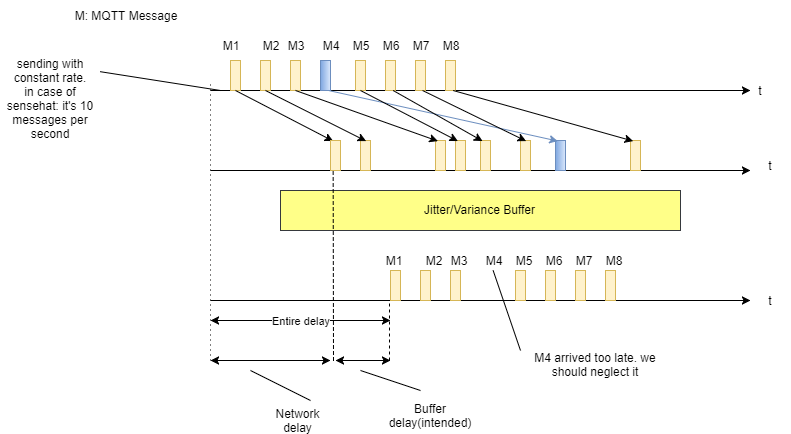
\includegraphics[width=1\linewidth]{jitter.png}
	\centering
	\caption{Jitter buffer}
	\label{fig:jitter.jpg}
\end{figure}
Another issue, in our code is that for each message we receive we have a time stamp (time stamp at the destination) and we add also a message number. But the trick is that we have noticed the time stamp in the message payload (the source time stamp) are in some cases earlier than the time stamp that we have created at the receiving point.\newline
A good solution would be to sync your clock at the sender and the receiver when you start your connection. We have to look at a solution that could operate at milisecond accuracy. ITP (internet time protocol) could be a solution but we are not sure.\newline
A furthermore problem is how we could improve the visualization of the wheel. It could be better in future work to use Simulink\footnote{\url{https://de.mathworks.com/videos/series/getting-started-with-simulink-3d-animation-94454.html}} and especial the library (3D animation). We are not sure if it's possible to do it with the current code. Any way, you could manipulate the java code.
\newline
The last point we have to announce is Octave\footnote{\url{https://www.gnu.org/software/octave/}}. This open source program is a possible alternative to Matlab that has similar capabilities and a similar programming language syntax. Because of this, Matlab code often can be executed using Octave. We could not guarantee that our program could work in octave and we didn't tested it there. 
\newpage
\section{Attachment}\label{sec:attachment}
\subsection{Source Code Node-red SensorTag}\label{sec:source-code-node-red SensorTag}
\lstinputlisting{sourcecodenodered.txt} 
\subsection{Source Code Node-red Sense-HAT}\label{sec:source-code-node-red Sense-HAT}
\lstinputlisting{sourcecodenoderedSense-HAT.txt} 

\subsection{Source Code Timestamp-node}\label{sec:source-code-timesptamp-node}
msg.payload=JSON.stringfy(msg.payload)+"-" +newDate().toString();\newline
return msg;
\subsection{How to write a simple MQTT Client in Java  with NetBeans}\label{sec:java-mqtt-client-and-its-main-method-in-matlab}

At first we searched for a way how we can get our data over MQTT into Matlab. We have found Paho\footnote{\url{http://www.eclipse.org/paho/}} as a suitable solution. The Eclipse Paho project provides open-source client implementations of MQTT and MQTT-SN messaging protocols aimed at new, existing, and emerging applications for the Internet of Things (IoT).
So it was nearly perfect for our purpose. In the following we explain the steps it takes to run an MQTT Client an its main method in Matlab:
\newline
\newline
\fbox{\begin{minipage}{35em}
		Download Paho eclipse MQTT Library (as a .jar file) from its eclipse paho repository: 
		\begin{itemize}
			\item Create a new java application project in your IDE such as eclipse.
			\item Add the .jar library to your project
		\end{itemize}
\end{minipage}}
\begin{verbatim}
our_project>properties>libraries>add a .jar file
\end{verbatim}
\fbox{\begin{minipage}{35em}
		Create a new class with name: 'SimpleMqttClient' inside the main method and create a new mqtt client:
\end{minipage}}
\begin{lstlisting} 	
MqttClient client = new MqttClient( "tcp://broker.mqttdashboard.com:1883", MqttClient.generateClientId() , new MemoryPersistence() );
\end{lstlisting}
\fbox{\begin{minipage}{35em}
		Here you pass an ip or url for the broker, in this case: broker.mqttdashboard.com 
\end{minipage}}
\begin{lstlisting}	
Set the call back method:
client.setCallback(new MqttCallback() {
@Override
public void connectionLost(Throwable cause) {}
\end{lstlisting}
\fbox{\begin{minipage}{35em}
		Called when the client lost the connection to the broker
\end{minipage}}
\begin{lstlisting}
@Override
public void messageArrived(String topic, MqttMessage message) throws Exception {mess = new String (message.getPayload());} 
@Override
public void deliveryComplete(IMqttDeliveryToken token) {}
});
\end{lstlisting}
\fbox{\begin{minipage}{35em}
		Called when a outgoing publish is complete
\end{minipage}}
\newline
\fbox{\begin{minipage}{35em}
		Also you have to declare a static string variable (mess) 
		Create a get-method called: getmessage() to call it in Matlab and get the messages.
		Connect to the broker:
\end{minipage}}
\begin{verbatim}
client.connect();
\end{verbatim}
\fbox{\begin{minipage}{35em}
		Subscribe for a topic and pass the QoS(Quality of Service):
\end{minipage}}
\begin{verbatim}
client.subscribe("Student_first_topic", 1);
\end{verbatim}
\fbox{\begin{minipage}{35em}
		Do not forget to import any required class.
		Compile the project and find the .jar file in your project directory.
		Add the file to dynamic path of matlab as we have described in the previous steps.
\end{minipage}}
\begin{verbatim}
javaaddpath ('C:\Users\Student\Desktop\testmatlab1\testmatlab1.jar’)
\end{verbatim}
\fbox{\begin{minipage}{15em}
		Now create a new instance:
\end{minipage}}
\begin{verbatim}
Client= SimpleMqttClient
\end{verbatim}
\fbox{\begin{minipage}{15em}
		Call the main method:
\end{minipage}}
\begin{verbatim}
javaMethod('main', Client,' ')
\end{verbatim}
\fbox{\begin{minipage}{35em}
		The last command in Matlab is to invoke any method in Matlab. You pass the method-name as Chat vector in the first argument the object you have created as second argument (or the class name if the method was static) and the method arguments in the next fields. 
		Notice that if your method don’t has arguments you have to pass an empty array (zero dimension). 
\end{minipage}}

\newpage
\subsection{How to setup Java in Matlab}\label{sec:how-to-setup-java-in-matlab}

For our solution we choose Java to run the MQTT-Protocol with Matlab. 
To be able to run Java code in Matlab, you have to check Java-Version of your Computer and Java-Version of Matlab.
Here is how it's done:

\begin{itemize}
	
	\item Start Matlab to determine if and which Java-Version is running 
	\item Write following command into the Matlab console: version -java
	\item To check Java-Verison on your machine start command interface(cmd)and enter: java -version 
	\item If this command is not recognized this means that you have to install (Java development kit) JDK onto your machine.(We worked with Version 1.8.0-31)\footnote{\url{http://www.oracle.com/technetwork/java/javase/downloads/index.html}}
	\item If the output of previous commands gives you the same Java-Version, then skip this part and go straight to \ref{sec:how-to-add-java-class-to-matlab}. Otherwise take the next steps. 
	\item If not, or Matlab is giving you an error, you have to change the JVM inside Matlab. To do that, go through the following steps:
	\begin{itemize}
		\item Write into the console of Matlab the following command:	
		\newline		getenv MATLAB\_JAVA	
		\item If the value is empty( ‘ ‘ ) then you have to create a new MATLAB\_JAVA environment variable in your system properties. Therefore go to:
			\begin{itemize}
				\item System Properties
				\item Press Environment Variables...
				\item Press New...
				\item add Variable name, and Variable value as shown in figurea \ref{img:Set Java path}
				\item The system variable should be your JRE path.
				\item add with ok and restart your PC
			\end{itemize} 
	\end{itemize}
	\begin{figure}[H]
		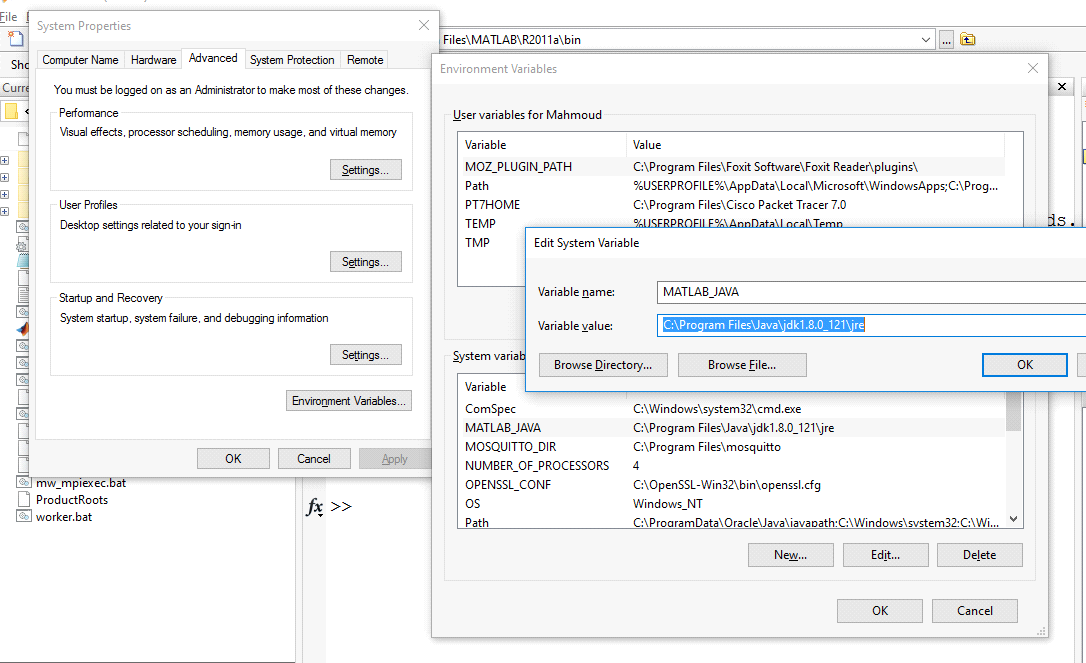
\includegraphics[width=\textwidth]{implent-java-matlab.png}
		\caption{Set Java path}
		\label{img:Set Java path}
	\end{figure}
	
	\item Check the value of MATLAB\_JAVA by writing the previous command in Matlab.
	Now check the Java-Version of your machine. It should be identical.
	
\end{itemize}

\subsection{How to add a Java class to Matlab}\label{sec:how-to-add-java-class-to-matlab}

Imagine you would like to use a Java file called test.java. First of all you have to write and compile this code by using either an IDE (eclipse or netbeans) or using the command line entering:
\begin{center}
	javac test.java 
\end{center} 
After compiling you get the file test.class. We are interested in this .class file. 
Now you have to add this .class file to your Matlab class path.
There are two ways: 
\begin{itemize}
	\item Add this file to the static class path
	\begin{itemize}
		\item Write into the console of Matlab \textless which classpath.txt\textgreater
		\item Now you get the directory where you could append your file to the static class file
		\item Just open the file as administrator and write at the end of the text the directory of your test.class file, e.g.:
		\begin{verbatim}
		C:\Users\Student\Desktop\testmatlab1
		\end{verbatim}
		\item Now you have to save the file and relaunch Matlab again.
		\item Declare in Matlab an instance of your class:
		\begin{verbatim}
		t = test 
		\end{verbatim} 
		\item if you get something like that: 
		\begin{verbatim}
		test@18c1ddd
		\end{verbatim}
		\item then you have successfully added a static class path
	\end{itemize}
	\item Adding your .class file to the dynamic path
	\begin{itemize}
		\item In this way you do not need system administrative privileges and you do not have to relaunch Matlab. It's also the solution we use in our program. 
		\item Just write the following command:
		\begin{verbatim}
		Javaaddpath ("write_here_your.class path")
		\end{verbatim}
		
		\item Example:
		
		\begin{center}
			\begin{verbatim}
			javaaddpath ('C:\Users\Student\Desktop\testmatlab1\testmatlab1.class') 
			\end{verbatim}
		\end{center}
		You also can add .jar files like this:
		\begin{center}
			\begin{verbatim}
			javaaddpath ('C:\Users\Student\Desktop\testmatlab1\testmatlab1.jar')
			\end{verbatim}
		\end{center}
		
		
		
	\end{itemize}
\end{itemize}

\subsection{Source Code Java - Main class}\label{sec:source-code-gui}
\lstset{language=Java} 
\lstset{basicstyle=\small}
\lstinputlisting{SourceCodeGUI.java} 
\newpage
\subsection{Source Code Java - Topic class}
\lstset{language=Java} 
\lstset{basicstyle=\small}
\lstinputlisting{topic.java} 
\end{document}
